%<<echo=FALSE>>=
%OLD <- options(width=90)
%@
%<<echo=FALSE>>=
%options(OLD) 
%@

\documentclass{beamer}\usepackage[]{graphicx}\usepackage[]{color}
%% maxwidth is the original width if it is less than linewidth
%% otherwise use linewidth (to make sure the graphics do not exceed the margin)
\makeatletter
\def\maxwidth{ %
  \ifdim\Gin@nat@width>\linewidth
    \linewidth
  \else
    \Gin@nat@width
  \fi
}
\makeatother

\definecolor{fgcolor}{rgb}{0.102, 0.102, 0.102}
\newcommand{\hlnum}[1]{\textcolor[rgb]{0.2,0.2,0.2}{#1}}%
\newcommand{\hlstr}[1]{\textcolor[rgb]{0.2,0.2,0.2}{#1}}%
\newcommand{\hlcom}[1]{\textcolor[rgb]{0.302,0.302,0.302}{\textit{#1}}}%
\newcommand{\hlopt}[1]{\textcolor[rgb]{0.102,0.102,0.102}{#1}}%
\newcommand{\hlstd}[1]{\textcolor[rgb]{0.102,0.102,0.102}{#1}}%
\newcommand{\hlkwa}[1]{\textcolor[rgb]{0.102,0.102,0.102}{#1}}%
\newcommand{\hlkwb}[1]{\textcolor[rgb]{0.102,0.102,0.102}{#1}}%
\newcommand{\hlkwc}[1]{\textcolor[rgb]{0.2,0.2,0.2}{#1}}%
\newcommand{\hlkwd}[1]{\textcolor[rgb]{0.102,0.102,0.102}{\textbf{#1}}}%

\usepackage{framed}
\makeatletter
\newenvironment{kframe}{%
 \def\at@end@of@kframe{}%
 \ifinner\ifhmode%
  \def\at@end@of@kframe{\end{minipage}}%
  \begin{minipage}{\columnwidth}%
 \fi\fi%
 \def\FrameCommand##1{\hskip\@totalleftmargin \hskip-\fboxsep
 \colorbox{shadecolor}{##1}\hskip-\fboxsep
     % There is no \\@totalrightmargin, so:
     \hskip-\linewidth \hskip-\@totalleftmargin \hskip\columnwidth}%
 \MakeFramed {\advance\hsize-\width
   \@totalleftmargin\z@ \linewidth\hsize
   \@setminipage}}%
 {\par\unskip\endMakeFramed%
 \at@end@of@kframe}
\makeatother

\definecolor{shadecolor}{rgb}{.97, .97, .97}
\definecolor{messagecolor}{rgb}{0, 0, 0}
\definecolor{warningcolor}{rgb}{1, 0, 1}
\definecolor{errorcolor}{rgb}{1, 0, 0}
\newenvironment{knitrout}{}{} % an empty environment to be redefined in TeX

\usepackage{alltt}% regular slides (with pauses)
%\documentclass[handout]{beamer}% handout (no pauses)

%%%%%%%%%%%%%%%%%%%%%%%%%%%%%%%%%%%%%%%%%%%%%%%%%%%%%%%%%%%%%%%%%%%%%%%%%
%%%%%%% Change the lecture information here %%%%%%%%%%%%%%%%
\def\chapnum{Week \#5}
\title{STAT234: Lecture 8 - Analyzing Tables}
\author{Kushal K. Dey}
\date{}
%%%%%%%%%%%%%%%%%%%%%%%%%%%%%%%%%%%%%%%%%%%%%%%%%%%%%%%%%%%%%%%%%%%%%%%%%

%%%%%% Start of suggested definitions and packages %%%%%%%%%%%%
%%%%%% Do not change unless you really know what you are doing %%%%%%%%%%
%%%%%%%%%%%%%%%%%%%%%%%%%%%%%%%%%%%%%%%%%%%%%%%%%%%%%%%%%%%%%%%%%%%%%%%%%

\usepackage{enumerate}
\usepackage{amsmath, bbm}
\usepackage[misc]{ifsym} % for the dice symbol \Cube{}
\usepackage[latin1]{inputenc}
\usepackage{hyperref}
\usepackage{multirow}

%\usepackage{comment}
%\usepackage{pstricks}
%\usepackage{graphicx}
%\usepackage{booktabs}
%\usepackage{pgfpages}
%\pgfpagesuselayout{2 on 1}[a4paper,border shrink=3mm]
%\pgfpagesuselayout{4 on 1}[a4paper,landscape,border shrink=3mm

\usepackage{setspace}
\ifdefined\knitrout
  \renewenvironment{knitrout}{\begin{spacing}{0.75}\begin{tiny}}{\end{tiny}\end{spacing}}
\else
\fi

%%%%%%%%%%%%%%% Defined Shortcuts (macros) %%%%%%%%%%%%%
% parameters and statistics
\newcommand{\xbar}{\overline{x}}
\newcommand{\Xbar}{\overline{X}}
\newcommand{\ybar}{\overline{y}}
\newcommand{\Ybar}{\overline{Y}}
\newcommand{\dbar}{\overline{d}}
\newcommand{\Dbar}{\overline{D}}
\newcommand{\zbar}{\overline{z}}
\newcommand{\Zbar}{\overline{Z}}
\newcommand{\ehat}{\widehat{\epsilon}}
\newcommand{\yhat}{\widehat{y}}
\newcommand{\Yhat}{\widehat{Y}}
\newcommand{\betaa}{{\beta_0}}
\newcommand{\betab}{{\beta_1}}
\newcommand{\betac}{{\beta_2}}
\newcommand{\betad}{{\beta_3}}
\newcommand{\BETA}{{\boldsymbol\beta}}
\newcommand{\betahata}{\widehat{\beta_0}}
\newcommand{\betahatb}{\widehat{\beta_1}}
\newcommand{\betahatc}{\widehat{\beta_2}}
\newcommand{\betahatd}{\widehat{\beta_3}}
\newcommand{\bhat}{\widehat{b}}
\newcommand{\btilde}{\widetilde{b}}
\newcommand{\ahat}{\widehat{a}}
\newcommand{\atilde}{\widetilde{a}}
\newcommand{\rss}{\mathit{SSE}}
\newcommand{\sigmahat}{\widehat{\sigma}}
\newcommand{\betahat}{\widehat{\beta}}
\newcommand{\thetahat}{\widehat{\theta}}
\newcommand{\phat}{\widehat{p}}
\newcommand{\pihat}{\widehat{\pi}}
\newcommand{\muhat}{\widehat{\mu}}
% real numbers and integers
\newcommand{\reals}{\mathbbm{R}}
\newcommand{\integers}{\mathbbm{N}}
%distributions
\newcommand{\normal}{\textsf{Norm}}
\newcommand{\Bin}{\textsf{Binom}}
\newcommand{\Uni}{\textsf{Unif}}
\newcommand{\Poisson}{\textsf{Pois}}
\newcommand{\Exp}{\textsf{Exp}}
\newcommand{\Beta}{\textsf{Beta}}
\newcommand{\iid}{\stackrel{\mathrm{iid}}{\sim}}
% probability and expected value
\newcommand{\rv}{r.v.\ }
\newcommand{\prob}{{\rm P}}
\newcommand{\mean}{\mathrm{E}}
\newcommand{\var}{\mathrm{Var}}
\newcommand{\Var}{\mathrm{Var}}
\newcommand{\cov}{\mathrm{Cov}}
\newcommand{\corr}{\mathop{\mathrm{Corr}}}
% measures of spread
\newcommand{\IQR}{\textit{IQR}}
\newcommand{\SAD}{\textit{SAD}}
\newcommand{\MAD}{\textit{MAD}}
\newcommand{\SSD}{\textit{SSD}}
\newcommand{\MSD}{\textit{MSD}}
\newcommand{\RMSD}{\textit{RMSD}}
\newcommand{\MSE}{\textit{MSE}}
\newcommand{\MSR}{\textit{MSR}}
% formatting code and such
\providecommand{\variable}[1]{}
\renewcommand{\variable}[1]{{\color{green!50!black}\texttt{#1}}}
\providecommand{\function}[1]{}
\renewcommand{\function}[1]{{\color{purple!75!blue}\texttt{\StrSubstitute{#1}{()}{}()}}}
\providecommand{\option}[1]{}
\renewcommand{\option}[1]{{\color{brown!80!black}\texttt{#1}}}
\providecommand{\pkg}[1]{}
\renewcommand{\pkg}[1]{{\color{red!80!black}\texttt{#1}}}
\providecommand{\code}[1]{}
\renewcommand{\code}[1]{{\color{blue!80!black}\texttt{#1}}}

%%%%%%%%%
% Changed by Kushal K Dey, University of Chicago
%\providecommand{\file}[1]{}
%\renewcommand{\file}[1]{{\tt #1}}
\providecommand{\file}[1]{}
\renewcommand{\file}[1]{{\color{orange!80!black}\texttt{#1}}}
%\providecommand{\dataframe}[1]{}
%\renewcommand{\dataframe}[1]{{\color{blue!80!black}\texttt{#1}}}
\providecommand{\dataframe}[1]{}
\renewcommand{\dataframe}[1]{{\color{cyan!80!black}\texttt{#1}}}
%%%%%%%%%

% other
\def\Sum{\sum\nolimits}
\def\b#1{\fboxsep=0pt\colorbox{black}{\color{white}\Cube{#1}}}
\def\w#1{\Cube{#1}}
%%%%%%%%%%%% End of shortcuts (macros) ##############

%%%%%%%%% One way to hide answers until you want to show them %%%%%%%%%
\def\Hide#1#2{\ul{~~~\onslide<#1>{\alert{#2}}~~~}}
\def\hide#1#2{\ul{~~\onslide<#1>{\alert{#2}}~~}}
\def\hid#1#2{\onslide<#1>{\alert{#2}}}
% Choose the color of answers here too
\setbeamercolor{alerted text}{fg=darkgray} 
%\setbeamercolor{alerted text}{fg=black} 

%------Centered Page Number Setup ------
\defbeamertemplate{footline}{centered page number}
{%
  \hspace*{\fill}%
  %\usebeamercolor[fg]{page number in head/foot}%
  %\usebeamerfont{page number in head/foot}%
  \tiny \chapnum: Page \insertframenumber\, of \inserttotalframenumber%
  \hspace*{\fill}\vskip2pt%
}
%\setbeamertemplate{footline}{\hfill\insertframenumber/\inserttotalframenumber}
\setbeamertemplate{footline}[centered page number]
%--------------------------------

%\usetheme{Copenhagen}
\setbeamertemplate{navigation symbols}{}
\usepackage[english]{babel}
\def\ul{\underline}
\linespread{1.1}
% or whatever



%\parskip=0pt
\IfFileExists{upquote.sty}{\usepackage{upquote}}{}
\begin{document}%large

%<<setup, include=FALSE, cache=FALSE>>=
%options(replace.assign=TRUE,width=90, digits=4)
%opts_chunk$set(fig.path='figure/graphics-', cache.path='cache/graphics-', fig.align='center', fig.width=8, fig.height=4.5, fig.show='as.is', out.width='0.9\\linewidth', cache=FALSE, par=TRUE, size = 'tiny', tidy=TRUE, cache.extra=rand_seed)
%knit_hooks$set(par=function(before, options, envir){
%if (before && options$fig.show!='none') par(mar=c(4,4,.1,.1),cex.lab=.95,cex.axis=.9,mgp=c(2,.7,0),tcl=-.3)
%}, document = function(x) {
%  gsub('\\\\(begin|end)\\{kframe\\}', '', x)
%}, crop=hook_pdfcrop)
%@
%<<setup2, include=FALSE, cache=FALSE>>=
%knit_theme$set("print")
%@


%%%%%%%%%%%%%%%%%%%%%%%%%%%%%%%%%%%%%%%%%%%%%%%%%%%%%%%%%%%%%%%%%%%%%%%%%
%%%%%%%%%%%%%%%%%%%%%%%%%%%%%%%%%%%%%%%%%%%%%%%%%%%%%%%%%%%%%%%%%%%%%%%%%
%%%%%% End of suggested definitions and packages %%%%%%%%%%%%

%------------------------------------------------------------------
%------------------------------------------------------------------

%%%%%%%%%% Title frame (optional) %%%%%%%%%%%%%
\begin{frame}{}
\maketitle
\end{frame}
%%%%%%%%%%%%%%%%%%%%%%%%%%%%%%%%%%%%%%%%%%%%%%%

%%%%%%%%%%%%%% Begin slides here %%%%%%%%%%%%%%

%%%%%%%%%%%%%%%%%%%%%%%%%%%%%%%%%%%%%%%%%%%%%%%
\begin{frame}[fragile]{Tables}
%%%%%%%%%%%%%%%%%%%%%%%%%%%%%%%%%%%%%%%%%%%%%%%

Early in this course, we talked about contingency tables. \pause  \newline

An example -  Yawning Contagious \pause


\begin{knitrout}\small
\definecolor{shadecolor}{rgb}{1, 1, 1}\color{fgcolor}\begin{kframe}
\begin{alltt}
\hlstd{yawn.data} \hlkwb{<-} \hlkwd{matrix}\hlstd{(}\hlkwd{c}\hlstd{(}\hlnum{10}\hlstd{,}\hlnum{4}\hlstd{,}\hlnum{24}\hlstd{,}\hlnum{12}\hlstd{),} \hlkwc{nrow}\hlstd{=}\hlnum{2}\hlstd{,} \hlkwc{byrow}\hlstd{=}\hlnum{TRUE}\hlstd{,}
                \hlkwc{dimnames} \hlstd{=} \hlkwd{list}\hlstd{(}\hlkwd{c}\hlstd{(}\hlstr{"Yawned"}\hlstd{,} \hlstr{"No Yawn"}\hlstd{),}
                                \hlkwd{c}\hlstd{(}\hlstr{"Yawn Seed"}\hlstd{,} \hlstr{"No Seed"}\hlstd{)))}
\hlstd{thetable} \hlkwb{<-}  \hlkwd{addmargins}\hlstd{(yawn.data)}
\hlstd{thetable}
\end{alltt}
\begin{verbatim}
        Yawn Seed No Seed Sum
Yawned         10       4  14
No Yawn        24      12  36
Sum            34      16  50
\end{verbatim}
\end{kframe}
\end{knitrout}

\end{frame}
%%%%%%%%%%%%%%%%%%%%%%%%%%%%%%%%%%%%%%%%%%%%%%%

%%%%%%%%%%%%%%%%%%%%%%%%%%%%%%%%%%%%%%%%%%%%%%%
\begin{frame}[fragile]{Tables}
%%%%%%%%%%%%%%%%%%%%%%%%%%%%%%%%%%%%%%%%%%%%%%%

\centering \Huge{Is there any effect of planting yawn seed on yawning?}

\end{frame}
%%%%%%%%%%%%%%%%%%%%%%%%%%%%%%%%%%%%%%%%%%%%%%%

%%%%%%%%%%%%%%%%%%%%%%%%%%%%%%%%%%%%%%%%%%%%%%%
\begin{frame}[fragile]{Tables}
%%%%%%%%%%%%%%%%%%%%%%%%%%%%%%%%%%%%%%%%%%%%%%%

We already solved this problem before.... \pause \newline

But that was using shuffles, similar to resampling or bootstrapping concept. \pause \newline

How about using a theoretical model? \pause \newline

Our focus today - model based inference of tables.

\end{frame}
%%%%%%%%%%%%%%%%%%%%%%%%%%%%%%%%%%%%%%%%%%%%%%%

%%%%%%%%%%%%%%%%%%%%%%%%%%%%%%%%%%%%%%%%%%%%%%%
\begin{frame}[fragile]{Tables}
%%%%%%%%%%%%%%%%%%%%%%%%%%%%%%%%%%%%%%%%%%%%%%%

For the $34$ cases where yawn seed is planted, define random variables $X_1, X_2, \cdots, X_{34}$ such that  

\begin{align}
X_i & = 1 \; \; if \; person \; yawns \\
& = 0 \;\; if \; person \; does \; not \; yawn \\
\end{align} 

Let $p_1$ be the probability 

$$ p_1 = Pr [ a \; person \; yawns |  yawn \; seed \; is \; planted ] $$ 

then, 

$$ X_{i} \sim Bin (34, p_{1}) $$

The conditionality of yawn seed planted is there because all the $X_{i}$'s are generated conditional on yawn seed being planted.

\end{frame}
%%%%%%%%%%%%%%%%%%%%%%%%%%%%%%%%%%%%%%%%%%%%%%%


%%%%%%%%%%%%%%%%%%%%%%%%%%%%%%%%%%%%%%%%%%%%%%%
\begin{frame}[fragile]{Tables}
%%%%%%%%%%%%%%%%%%%%%%%%%%%%%%%%%%%%%%%%%%%%%%%

For the $16$ cases where yawn seed is not planted, define random variables $Y_1, Y_2, \cdots, Y_{16}$ such that  

\begin{align}
Y_i & = 1 \; \; if \; person \; yawns \\
& = 0 \;\; if \; person \; does \; not \; yawn \\
\end{align} 

Let $p_2$ be the probability 

$$ p_2 = Pr [ a \; person \; yawns |  yawn \; seed \; is \; not \; planted ] $$ 

then, 

$$ Y_{i} \sim Bin (16, p_{2}) $$

The conditionality of yawn seed planted is there because all the $Y_{i}$'s are generated conditional on yawn seed being planted.

\end{frame}
%%%%%%%%%%%%%%%%%%%%%%%%%%%%%%%%%%%%%%%%%%%%%%%

%%%%%%%%%%%%%%%%%%%%%%%%%%%%%%%%%%%%%%%%%%%%%%%
\begin{frame}[fragile]{Tables}
%%%%%%%%%%%%%%%%%%%%%%%%%%%%%%%%%%%%%%%%%%%%%%%

We reduce a contingency table to a 2-sample problem 

$$ X_{1}, X_{2}, \cdots, X_{34} \sim Bin (34, p_1) $$
$$ Y_{1}, Y_{2}, \cdots, Y_{16} \sim Bin (16, p_2) $$ \pause

What is the hypothesis?

$$ H_{0}: p_{1} = p_{2}  \;\; H_{1}: p_{1} > p_{2} $$ \pause

$$ \hat{p}_{1} = \frac{10}{34} \;\; \hat{p}_{2} = \frac{4}{16}  $$ \pause

$$ \hat{p}_{1} - \hat{p}_{2} = \frac{10}{34} - \frac{4}{16} = 0.044 $$

\end{frame}
%%%%%%%%%%%%%%%%%%%%%%%%%%%%%%%%%%%%%%%%%%%%%%%

%%%%%%%%%%%%%%%%%%%%%%%%%%%%%%%%%%%%%%%%%%%%%%%
\begin{frame}[fragile]{Tables}
%%%%%%%%%%%%%%%%%%%%%%%%%%%%%%%%%%%%%%%%%%%%%%%

You know 

$$ E (\hat{p}_{1} - \hat{p}_{2}) = E(\hat{p}_1) - E(\hat{p}_2) = p_{1} - p_{2} $$ \pause

But to make inference on $p_{1} - p_{2}$, we need to know the distribution of $\hat{p}_{1} - \hat{p}_{2}$. 

We know under \textbf{large sample assumption}

$$ \hat{p}_{1} \sim N(p_1, \frac{p_1(1-p_1)}{34}) $$
$$ \hat{p}_{2} \sim N(p_2, \frac{p_2(1-p_2)}{16}) $$ 

Note that $X_{i}$ and $Y_{j}$ are all independent, hence so are $\hat{p}_{1}$ and $\hat{p}_{2}$.

$$ \hat{p}_{1} - \hat{p}_{2} \sim N \left( p_1 - p_2, \frac{p_1(1-p_1)}{34} + \frac{p_2(1-p_2)}{16} \right ) $$

\end{frame}
%%%%%%%%%%%%%%%%%%%%%%%%%%%%%%%%%%%%%%%%%%%%%%%

%%%%%%%%%%%%%%%%%%%%%%%%%%%%%%%%%%%%%%%%%%%%%%%
\begin{frame}[fragile]{Tables}
%%%%%%%%%%%%%%%%%%%%%%%%%%%%%%%%%%%%%%%%%%%%%%%

Under $H_{0}$, we have 

$$ p_{1} = p_{2} = p (say)$$

$$ \hat{p}_{1} - \hat{p}_{2} \sim N \left(0, \frac{p(1-p)}{34} + \frac{p(1-p)}{16} \right ) $$

$$ \frac{\hat{p}_{1} - \hat{p}_{2}}{\sqrt{\frac{p(1-p)}{34} + \frac{p(1-p)}{16}}} \sim N(0,1) $$


We replace $p$ by $\hat{p}$,

$$ \hat{p} = \frac{10+4}{36+14} = \frac{14}{50} $$

\end{frame}
%%%%%%%%%%%%%%%%%%%%%%%%%%%%%%%%%%%%%%%%%%%%%%%

%%%%%%%%%%%%%%%%%%%%%%%%%%%%%%%%%%%%%%%%%%%%%%%
\begin{frame}[fragile]{Tables}
%%%%%%%%%%%%%%%%%%%%%%%%%%%%%%%%%%%%%%%%%%%%%%%

under large sample assumption

$$ T = \frac{\hat{p}_{1} - \hat{p}_{2}}{\sqrt{\hat{p}(1- \hat{p}) (\frac{1}{34} + \frac{1}{16})}} \sim N(0,1) $$

We find the realized value of this quantity from the sample after substituting the values of $\hat{p}_{1} = \frac{10}{36} $, $\hat{p}_{2} = \frac{4}{16}$ and $\hat{p}= \frac{14}{50}$, \pause \newline

$$ t = 0.275 $$ \pause 

The p-value of this quantity

$$ Pr \left ( Z > t \right) = 0.4  >> 0.05$$ \pause 

We reject researchers' claim !!

\end{frame}
%%%%%%%%%%%%%%%%%%%%%%%%%%%%%%%%%%%%%%%%%%%%%%%


%%%%%%%%%%%%%%%%%%%%%%%%%%%%%%%%%%%%%%%%%%%%%%%
\begin{frame}[fragile]{Revisit Bootstrapping/ Resampling}
%%%%%%%%%%%%%%%%%%%%%%%%%%%%%%%%%%%%%%%%%%%%%%%

We generate $N \hat{p} = 50 \times \frac{14}{50} = 14$ cards which are red (yawners) and $N \times (1- \hat{p}) = 36$ cards which are black (non-yawners). \pause \newline

Shuffle the pile of cards. \pause \newline

Take $34$ cards from the pile and calculate the number of red cards (these are my $X$) \pause 
\newline

Take $16$ cards from remaining pile and calculate the number of red cards (these are my $Y$).
\pause \newline

\end{frame}
%%%%%%%%%%%%%%%%%%%%%%%%%%%%%%%%%%%%%%%%%%%%%%%



%%%%%%%%%%%%%%%%%%%%%%%%%%%%%%%%%%%%%%%%%%%%%%%
\begin{frame}[fragile]{Revisit Bootstrapping/ Resampling}
%%%%%%%%%%%%%%%%%%%%%%%%%%%%%%%%%%%%%%%%%%%%%%%

Calculate proportion of red cards in each of th two draws $\hat{p}_{1}$ and $\hat{p}_{2}$ anc calculate $\hat{p}_{1} - \hat{p}_{2}$. \pause \newline

Repeat this $1000$ times and record the number of times we get the value of $\hat{p}_{1} - \hat{p}_{2}$ greater than $0.044$. Thats my p-value \pause \newline

This is equivalent to construct the histogram of $\hat{p}_{1} - \hat{p}_{2}$ values from the $10000$ draws and counting the frequencies above $0.044$

\end{frame}
%%%%%%%%%%%%%%%%%%%%%%%%%%%%%%%%%%%%%%%%%%%%%%%


%%%%%%%%%%%%%%%%%%%%%%%%%%%%%%%%%%%%%%%%%%%%%%%
\begin{frame}[fragile]{Summary}
%%%%%%%%%%%%%%%%%%%%%%%%%%%%%%%%%%%%%%%%%%%%%%%

We saw how one can test for effectiveness of a hypothesis from contingency table.  \pause \newline

The Normal test is only applicable for large number of samples \pause \newline

The Bootstrap/Resampling test does not assume distribution but will give different results over different runs \pause \newline

But this was for a $2 \times 2$ table. Can we have a test for a table with 3 or more categories?  \pause \newline

\end{frame}
%%%%%%%%%%%%%%%%%%%%%%%%%%%%%%%%%%%%%%%%%%%%%%%

%%%%%%%%%%%%%%%%%%%%%%%%%%%%%%%%%%%%%%%%%%%%%%%
\begin{frame}[fragile]{Chi-square table}
%%%%%%%%%%%%%%%%%%%%%%%%%%%%%%%%%%%%%%%%%%%%%%%


\begin{knitrout}\small
\definecolor{shadecolor}{rgb}{1, 1, 1}\color{fgcolor}\begin{kframe}
\begin{alltt}
\hlstd{yawn.data} \hlkwb{<-} \hlkwd{matrix}\hlstd{(}\hlkwd{c}\hlstd{(}\hlnum{10}\hlstd{,}\hlnum{4}\hlstd{,}\hlnum{24}\hlstd{,}\hlnum{12}\hlstd{),} \hlkwc{nrow}\hlstd{=}\hlnum{2}\hlstd{,} \hlkwc{byrow}\hlstd{=}\hlnum{TRUE}\hlstd{,}
                \hlkwc{dimnames} \hlstd{=} \hlkwd{list}\hlstd{(}\hlkwd{c}\hlstd{(}\hlstr{"Yawned"}\hlstd{,} \hlstr{"No Yawn"}\hlstd{),}
                                \hlkwd{c}\hlstd{(}\hlstr{"Yawn Seed"}\hlstd{,} \hlstr{"No Seed"}\hlstd{)))}
\hlstd{O} \hlkwb{<-}  \hlkwd{addmargins}\hlstd{(yawn.data)}
\hlstd{O}
\end{alltt}
\begin{verbatim}
        Yawn Seed No Seed Sum
Yawned         10       4  14
No Yawn        24      12  36
Sum            34      16  50
\end{verbatim}
\end{kframe}
\end{knitrout}
\pause
What would be expected counts under the null, if we assume $p_{1}=p_{2}=p$, we should have

\begin{tabular}{|c|c|c|c|}
& Yawned & No Yawn & Total\\ \hline
Yawn Seed & $34 \times p$ & $16 \times p$  & $50 \times p$ \\ \hline
No seed & $34 \times (1-p)$ & $16 \times (1-p)$ & $50 \times (1-p)$ \\ \hline
Total  & 34 & 16 & 50  \\ \hline 
\end{tabular}

\end{frame}
%%%%%%%%%%%%%%%%%%%%%%%%%%%%%%%%%%%%%%%%%%%%%%%

%%%%%%%%%%%%%%%%%%%%%%%%%%%%%%%%%%%%%%%%%%%%%%%
\begin{frame}[fragile]{Chi-square table}
%%%%%%%%%%%%%%%%%%%%%%%%%%%%%%%%%%%%%%%%%%%%%%%

Since we do not know $p$, we replace it by $\hat{p}$.

$$ \hat{p} = 14/50 $$ \pause

The table under the null expected then is

\begin{knitrout}\small
\definecolor{shadecolor}{rgb}{1, 1, 1}\color{fgcolor}\begin{kframe}
\begin{alltt}
\hlstd{yawn.data} \hlkwb{<-} \hlkwd{matrix}\hlstd{(}\hlkwd{c}\hlstd{(}\hlnum{9.52}\hlstd{,}\hlnum{4.48}\hlstd{,}\hlnum{24.48}\hlstd{,}\hlnum{11.52}\hlstd{),} \hlkwc{nrow}\hlstd{=}\hlnum{2}\hlstd{,} \hlkwc{byrow}\hlstd{=}\hlnum{TRUE}\hlstd{,}
                \hlkwc{dimnames} \hlstd{=} \hlkwd{list}\hlstd{(}\hlkwd{c}\hlstd{(}\hlstr{"Yawned"}\hlstd{,} \hlstr{"No Yawn"}\hlstd{),}
                                \hlkwd{c}\hlstd{(}\hlstr{"Yawn Seed"}\hlstd{,} \hlstr{"No Seed"}\hlstd{)))}
\hlstd{E} \hlkwb{<-}  \hlkwd{addmargins}\hlstd{(yawn.data)}
\hlstd{E}
\end{alltt}
\begin{verbatim}
        Yawn Seed No Seed Sum
Yawned       9.52    4.48  14
No Yawn     24.48   11.52  36
Sum         34.00   16.00  50
\end{verbatim}
\end{kframe}
\end{knitrout}


\end{frame}
%%%%%%%%%%%%%%%%%%%%%%%%%%%%%%%%%%%%%%%%%%%%%%%

%%%%%%%%%%%%%%%%%%%%%%%%%%%%%%%%%%%%%%%%%%%%%%%
\begin{frame}[fragile]{Chi-square table}
%%%%%%%%%%%%%%%%%%%%%%%%%%%%%%%%

Take the observed table $O$ and the expected table $E$. If the null hypothesis is not true, we will expect the squared differences $$ (O_{ij} - E_{ij})^2 $$ to be high (i=1,2 , j=1,2). \pause

Lets consider the expression 

$$ X = \sum_{i,j} \frac{(O_{ij}-E_{ij})^2}{E_{ij}} $$

We need  distribution for  $X$. This distribution has a fancy name - \textbf{Chi-square distribution} with degrees of freedom $(r-1) \times (c-1)$ where $r$ is the number of rows in table and $c$ is the number of columns. 

$$  X \sim \chi^2_{(2-1)(2-1))} = \chi^2_{1} $$

\end{frame}
%%%%%%%%%%%%%%%%%%%%%%%%%%%%%%%%%%%%%%%%%%%%%%%

%%%%%%%%%%%%%%%%%%%%%%%%%%%%%%%%%%%%%%%%%%%%%%%
\begin{frame}{Chi-Square Distribution}
%%%%%%%%%%%%%%%%%%%%%%%%%%%%%%%%%%%%%%%%%%%%%%%

The chi-square distributions: $\chi_k^2$
$$f(x) = \frac{ x^{(k/2)-1} e^{- x/2}}{2^{k/2}\Gamma(k/2)}
  \qquad x>0,\, k\geq 1$$ \pause
$$E(X) = k \qquad Var(X) = 2k$$ \pause

\begin{center}
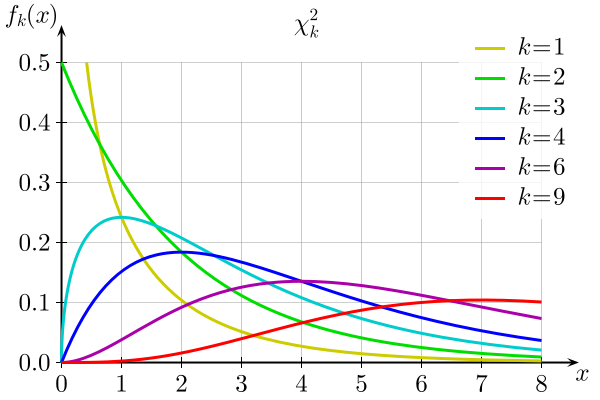
\includegraphics[width=8cm,height=4cm]{chi-square.png}
\end{center}


\end{frame}
%%%%%%%%%%%%%%%%%%%%%%%%%%%%%%%%%%%%%%%%%%%%%%%


%%%%%%%%%%%%%%%%%%%%%%%%%%%%%%%%%%%%%%%%%%%%%%%
\begin{frame}{Chi-Square Distribution}
%%%%%%%%%%%%%%%%%%%%%%%%%%%%%%%%%%%%%%%%%%%%%%%

The chi-square distributions: $\chi_1^2$
$$f(x) = \frac{ x^{-1/2} e^{- x/2}}{\sqrt{2\pi}}
  \qquad x>0$$ \pause
  
Origin of the Chi-square distribution: \\
Let $Z\sim N(0,1)$ and define $Y=Z^2.$  Then, $Y\sim \chi^2_1.$ \pause
\bigskip



\bigskip
In general, $\chi_n^2$ is a sum of $n$ i.i.d. standard normal distributions.

  \end{frame}
%%%%%%%%%%%%%%%%%%%%%%%%%%%%%%%%%%%%%%%%%%%%%%%





\end{document}
